\section{EAP Method Definition}
\label{section:eap-84-definition}
We want to encapsulate our extended zero-knowledge authentication system defined in \S\ref{label:protocol-design} as an EAP method in the EAP framework we've explored in \S\ref{section:eap}.
To achieve this, we must define a new EAP method, which comprises of the messages exchanged between the \textit{peer} and the \textit{authenticator}, their data formats and the processes for handling them.

\paragraph{Terminology.}
In this section we will use EAP terminology as described in \S\ref{section:eap}, which uses different names to describe parties involved, as the ones used in our system architecture in \S\ref{label:protocol-design} or as in the ZKP protocol in \S\ref{zkp-qrp}.
The two parties in EAP are called the peer and the authenticator, where the peer is authenticating with the authenticator.
To draw parallels between our system architecture, where we use the names \textit{user} and \textit{authentication system}, the peer is the user, and the authenticator is the authentication system.
In the ZKP protocol names \textit{prover} and \textit{verifier} are used, the peer is the prover, and the authenticator is the verifier.

\bigskip
\noindent
To define an EAP method, we need to break down our authentication system described in \S\ref{label:protocol-design} to EAP messages representing interactions between the user and the authentication system.
Each message defines its data format, the sender and recipient processes and local state changes.
Our EAP method defines two messages, the \textit{setup phase} message and the \textit{verification phase} message.

We designed our authentication system for multiple users. 
For this reason, the authenticator needs to start the authentication process with the \textit{identification phase} by querying the identity of the peer with the \textit{identity} (Type 1) EAP message as described in \S\ref{def:eap-identitiy}.
In the \textit{setup phase} the peer uses the \textit{setup} message for discovery of ZKP parameters, and to provide the values for the first proof verification round to the authenticator.
This message is exchanged only once.
In the \textit{verification phase} the \textit{verification} message is used to exchange data required for a single round of proof verification. Since proof verification as described in \S\ref{zkp-qrp} requires $m$ iterations, this message is exchanged $m$ times.
The protocol ends with the authenticator sending either a \textit{success} or a \textit{failure} message.

\subsubsection{Authentication process overview}
Let us examine the EAP messages (Figure \ref{fig:eap-84}) of the authentication process described in Table \ref{table:zkp-qrp-2}.
The mapping between EAP messages and the steps in Table \ref{table:zkp-qrp-2} is \textit{not one-to-one}, as we merged some steps to reduce the number of message exchanges to speed up the whole process.
In this section we present a simplified authentication process to present the general idea, while a detailed description is given in the next section.

The mathematical variables have the same meaning as in the system architecture described in \S\ref{label:protocol-design}. This applies to all further sections.
\begin{table}[h!]
	\centering
	\caption{Improved ZKP Authentication with EAP}
	\vspace{0.2cm}
	\begin{tabular}{l|l|c|l}
  		& Peer & & Authenticator\\
  		\hline
  		1 & & $\xrightarrow{I}$ &\\
		2 & $w = H(p, s)$ & $\xleftarrow{s,n}$ & \\
		\hline
		3 & $u_i \leftarrow_R \Bbb{Z}_{n}$ &  \\
		& $y_i = u_i^2 \Mod{n}$ & $\xrightarrow{y_i}$ \\
		4 & & $\xleftarrow{b_i}$ & $b_i \leftarrow_R \{0, 1\} $ \\
		5 & $z_i = u_iw^{b_i} \Mod n $ & $\xrightarrow{z_i}$ & check $z_i^2 \equiv y_ix^{b_i} \Mod{n}$\\
	\end{tabular}
	\label{table:zkp-qrp-2}
\end{table}

\begin{figure}[h!]
	\centering
	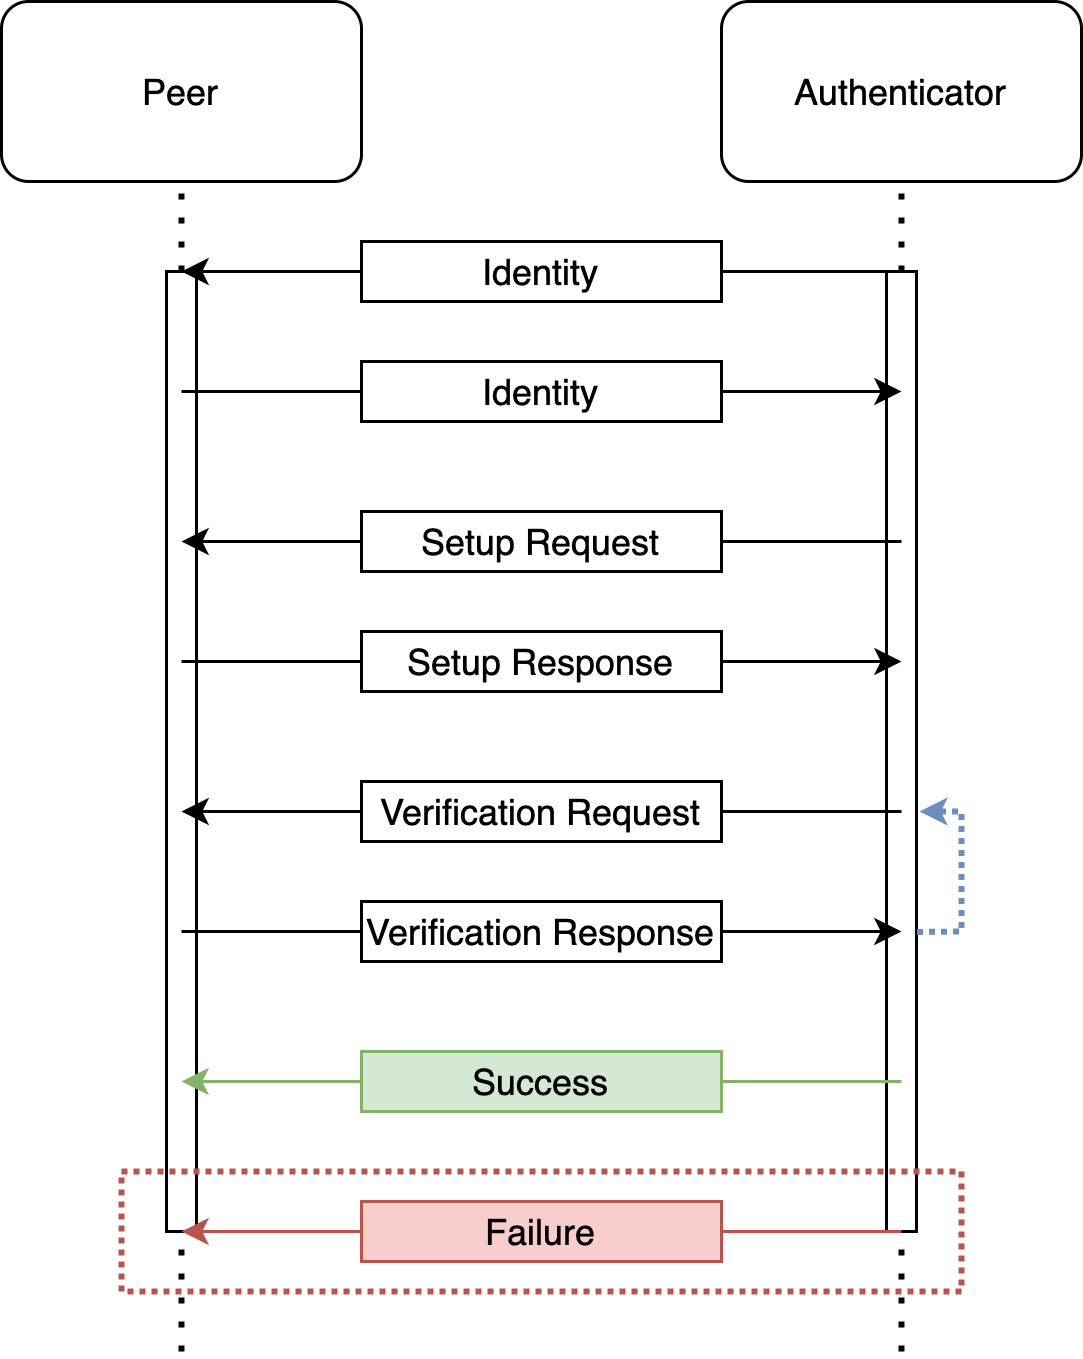
\includegraphics[width=14cm]{images/eap-zkp}
	\caption{EAP Method Execution}
	\label{fig:eap-84}
\end{figure}

The authentication process (Figure \ref{fig:eap-84}) consists of multiple phases:

\begin{description}
	\item [Identification Phase] Used to establish the identity of the peer. The authenticator sends an \textit{identity request} message, and the peer responds with an identifier $I$, which is used the locate the salt $s$ and quadratic residue value $x$. (Table \ref{table:zkp-qrp-2}, Step 1.)
	\item [Setup Phase] Used to exchange necessary values for the \textit{verification phase}. The authenticator sends the salt $s$ and modulus $n$ in the \textit{setup request} message, which the peer uses to derive the root $w$ from the password $p$. The peer responds with $y_1$ which will be used in the first round of the verification phase. (Table \ref{table:zkp-qrp-2}, Steps 2. and 3.)
	\item [Verification Phase] In this phase both parties continuously exchange data for $m$ rounds to construct and verify the proof. In a given round $i$ the authenticator sends the random bit $b_i$ and the peer responds with the partial proof $z_i$. The peer also sends the $y_{i+1}$ for the next verification round $i+1$, this is done as a performance optimization (Table \ref{table:zkp-qrp-2}, Steps 4., 5. and 3. again). After receiving each response the authenticator verifies the partial proof, once he has done so for $m$ successfully, he sends a \textit{success} message. If the partial proof isn't valid, the authenticator must send a \textit{failure} message.
\end{description}

\subsubsection{Message Format}

\begin{center}
\begin{tabular}{|c|c|c|c|}
	\hline
	Length (Octets) & 1 & $k$\\
	\hline
	Field & Phase Type & Phase Data\\
	\hline
\end{tabular}
\end{center}

\noindent
An EAP message is composed of many fields (Table \ref{table:eap-message}).
The \textit{type} field as described in \S\ref{text:eap:type} determines the EAP method used by the peer and the authenticator to interpret the \textit{type-data} field.
Our EAP method is indicated with \textit{type} value $84$.

The \textit{type-data} field is composed of two sub fields, a \textit{phase type} field and a \textit{phase data} field.
\textit{Phase} identifies the phase of the authentication process, while \textit{phase data} holds specific data for that phase.
We have defined 2 \textit{phase} values, that correspond with the phases of our authentication process:

\begin{quote}
	\begin{description}
		\item [Phase Type 1]: Setup Message (Figure \ref{fig:eap-84} - Setup Phase)
		\item [Phase Type 2]: Verification Message (Figure \ref{fig:eap-84} - Verification Phase)
	\end{description}
\end{quote}

The \textit{Identification Phase} in Figure \ref{fig:eap-84} doesn't have a corresponding \textit{phase type} value as the \textit{Identity} message as described in \S\ref{def:eap-identitiy} is a pre-defined EAP message type.

Note also, that the architecture does not specify a key-stretching method, and neither does this EAP method.
We assume that in a practical implementation the method would be pre-defined and implicitly known by both parties.

\subsection{Setup Phase}
Previously we assumed the modulus $n$ and salt $s$ are known by the user, however, the EAP method needs to facilitate the discovery of this data.
Our system is designed to support multiple users, so before this phase the authenticator needs to identify the peer with the \textit{identity} message.
The response message additionally contains the control value $y_1$, used to verify the proof in the first verification round. The data is already included in this message to improve the method performance.

\subsection*{Request Message} Message is used to deliver the salt $s$ and semiprime modulus $n$ to the peer.

\paragraph{Phase Data Format}

\begin{center}
\begin{tabular}{|c|c|c|c|}
	\hline
	Length (Octets) & 1 & $4 \le k \le 255 $ & $64 \le j$\\
	\hline
	Field & Salt Length & Salt & Modulus\\
	\hline
\end{tabular}
\end{center}

\begin{quote}
\begin{description}
	\item[Salt Length] A single octet for the length of the \textit salt field in octets.
	\item[Salt] A random salt value, should be from 4 octets to 255 octets long.
The max length is determined by the largest number able to be encoded in the \textit {salt length} field.
	\item[Modulus] Fills the rest of the message to the length specified by the \textit{length} field in the EAP message. 
Should be at least 64 octets (512 bits).
\end{description}
\end{quote}

\paragraph{Request Handling} When a request is received, the peer computes the root $w$ using the password $p$ the salt $s$ with the pre-determined hashing function $H$.
Root $w$ should be stored stored in memory by the peer. 
Next the peer should pick a random integer $u$ from field $Z^*_n$, and store it in memory and then computes the control value $y = u^2 \Mod{n}$.
The control value $y$ is included in the response message.

\subsection*{Response Message}
The response contains the control value $y_1$ to the authenticator to be used in the first round of the verification process.
The subscript of a variable $y_i$ denotes in which verification round $i$ is the variable used.

\paragraph{Phase Data Format}

\begin{center}
\begin{tabular}{|c|c|}
	\hline
	Length (Octets) & $k$ \\
	\hline
	Field & Control Value $y_1$\\
	\hline
\end{tabular}
\end{center}

\bigskip
\begin{quote}
\begin{description}
	\item[Control Value] Computed by the peer, where $y_1 = u_1^2 \Mod{n}$ and $u_1 \leftarrow_R \mathbb{Z}^*_n$.
\end{description}
\end{quote}

\paragraph{Response Handling}
The authenticator should store the $y_1$ control value locally to be used when verifying the proof $z_1$.

\subsection{Verification Phase}
This message pair exchanges data required to compute and verify the proof.
They continuously exchange it until the authenticator concludes the authentication.
After $m$ successful rounds, when the authenticator reaches a confidence of $1 - 2^{-m}$ in the proof, the authentication is successful.
To make our method more efficient, we reduce the number of exchanged messages between the parties by interlacing some data between iterations.
On the round $i$, the response contains data required for the round $i+1$.


\subsection*{Request Message}
In the round $i$, the authenticator generates random bit $b_i$ stores it locally, and sends it to the peer.
\paragraph{Message Data Format}

\begin{center}
\begin{tabular}{|c|c|}
	\hline
	Length (Octets)  & $1$ \\
	\hline
	Field & Random Bit $b_i$\\
	\hline
\end{tabular}
\end{center}

\begin{quote}
\begin{description}
	\item[Random Bit] A single-bit $b_i$, at the right-most place. 1 octet long.
\end{description}
\end{quote}

\paragraph{Request Handling}
The peer computes the proof $z_i = u_iw^{b_i} \Mod{n}$, with the bit $b_i$ received in the request.

Additionally the peer generates the control value $y_{i+1}$ for the next ($i+1$) verification round.
The peer picks a random integer $u_{i+1}$ from field $Z^*_n$ and stores it in memory.
The control value is computed as $y_{i+1} = u_{i+1}^2 \Mod{n}$ and sent in the response.

\subsection*{Response Message}
The response transmits the proof $z_i$ and the control value $y_{i+1}$ to the authenticator, who verifies the proof and decides on how to proceed.

\paragraph{Message Data Format}

\begin{center}
\begin{tabular}{|c|c|c|c|}
	\hline
	Length (Octets) & $1$ & $k $ & $j$\\
	\hline
	Field & Proof Length & Proof $z_i$ & Control Value $y_{i+1}$\\
	\hline
\end{tabular}
\end{center}

\begin{quote}
\begin{description}
	\item [Proof Length] A field one octet in length. Determines the length of the Proof field in octets.
	\item [Proof] Value $z_i$ computed by the peer, verified by the authenticator.
	\item [Control Value] Value $y_{i+1}$, required to verify the proof of the $(i+1)$-th round.
\end{description}
\end{quote}

\paragraph{Response Handling}
The authenticator should verify the proof by asserting that $z_i^2 \equiv y_ix^{b_i} \Mod{n}$.
If the verification fails, the a \textit{failure} message must be sent to the peer, otherwise a \textit{success} message must be sent if the verification was successful for $m$ rounds.
If that is not the case, the $y_{i+1}$ is stored by the authenticator and a new verification message request is sent.